% !TeX encoding = windows-1251
\documentclass[fullscreen=true,russian,compress,%
    hyperref={unicode,bookmarks=false}]{presentation}
\inputencoding{utf8}
\usepackage[russian]{babel}
\usepackage{paratype}
\makefootline{.35}{.55}{.1}

\usepackage{csquotes}
\usepackage{tikz}
\usetikzlibrary{arrows.meta, positioning, shapes.geometric}
\usepackage{booktabs}
\usepackage{array}
\usepackage{graphicx}
\graphicspath{{images/}}

\begin{document}

\title[Игровое приложение <<Коридор>>]{Разработка игрового приложения\\ <<Коридор>> с модулем стратегического поведения соперника}
\author{Александр Олегович Карпунин}
\institute{Научный руководитель: А.В. Николаев}
\date{2026}

\begin{frame}
\titlepage
\end{frame}

\section{Вступление}

\begin{frame}{Вступление}
\begin{block}{Цель работы}
Целью выпускной квалификационной работы является разработка игрового приложения <<Коридор>>, включающего в себя реализацию правил игры, визуализацию игрового поля и модуль стратегического поведения, объединяющий четыре алгоритма программного соперника.
\end{block}

\end{frame}

\begin{frame}{Задачи работы}
\begin{block}{Основные задачи}
\small
\begin{enumerate}
    \item изучить правила игры <<Коридор>>;
    \item реализовать алгоритм проверки корректности перемещения фишки;
    \item реализовать алгоритм проверки корректности установки перегородки с условием достижимости целевых сторон поля;
    \item реализовать алгоритм поиска кратчайшего пути до целевой стороны поля на основе обхода графа в ширину;
    \item разработать функцию оценки позиции игрока с настраиваемыми весами и механизмом их коррекции по результатам партий;
    \item реализовать четыре алгоритма программного соперника: случайный выбор хода, Минимакс, альфа-бета отсечение и Монте-Карло;
    \item провести сравнение алгоритмов в серии автоматических партий;
    \item разработать интерфейс игрового приложения.
\end{enumerate}
\end{block}
\end{frame}

\section{Игра}

\begin{frame}{Игра <<Коридор>>}
\begin{columns}
\begin{column}{.48\textwidth}
\begin{block}{Правила}
\begin{itemize}
    \item цель игрока "--- довести свою фишку до противоположной стороны игрового поля быстрее соперника;
    \item за ход можно передвинуть свою фишку или поставить стену, которая будет блокировать перемещение между соседними клетками;
    \item установленная стена не должна препятствовать достижению игроками их победных сторон поля;
    \item количество стен ограничено.
\end{itemize}
\end{block}
\end{column}
\begin{column}{.52\textwidth}
\begin{figure}
    \centering
    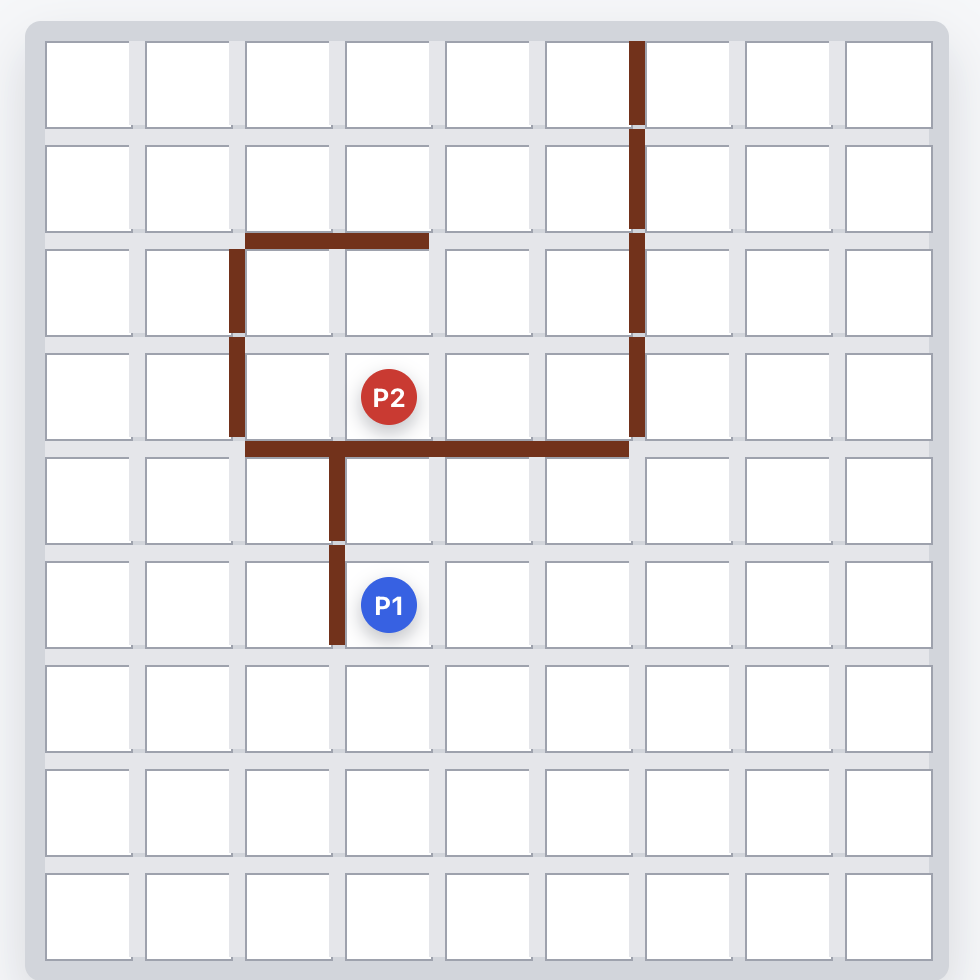
\includegraphics[width=.88\textwidth]{game-board.png}
\end{figure}
\end{column}
\end{columns}
\end{frame}

\section{Реализация}

\begin{frame}{Архитектура приложения}
\begin{figure}
\centering
\begin{tikzpicture}[
    box/.style={draw, rounded corners, align=center, minimum width=8.5cm, minimum height=.7cm},
    arrow/.style={-{Stealth[length=2.5mm]}, thick}
]
    \node[box] (ui) {UI Vaadin\\ StartPageController, GamePageController, TournamentPageController};
    \node[box, below=.45cm of ui] (service) {Сервисный слой\\ GameProcessor, GameRules, TournamentService, BoardAnalyzer};
    \node[box, below=.45cm of service] (alg) {Модуль алгоритмов\\ Random, MiniMax, AlphaBeta, MonteCarlo};
    \node[box, below=.45cm of alg] (model) {Игровая модель\\ Game, Board, Move, Position, Player};
    \node[box, below=.45cm of model] (data) {Файлы данных\\ evaluation-weights.properties};
    \draw[arrow] (ui) -- (service);
    \draw[arrow] (service) -- (alg);
    \draw[arrow] (alg) -- (model);
    \draw[arrow] (model) -- (data);
\end{tikzpicture}
\end{figure}
\end{frame}

\begin{frame}{Генерация допустимых ходов}
\begin{block}{Перемещение фишки}
Для текущей позиции строится множество доступных соседних клеток с учетом стен, границ поля, прыжков через соперника и диагональных прыжков при невозможности прямого прыжка.
\end{block}

\begin{block}{Установка стены}
Для стены проверяются пересечения, наличие стен у игрока и сохранение пути к целевой стороне для обоих игроков. Достижимость проверяется обходом графа в ширину.
\end{block}
\end{frame}

\begin{frame}{Функция оценки позиции}
\begin{block}{Общая форма}
\[
F(s)=\sum_i \lambda_i f_i(s)
\]
\end{block}

\begin{block}{Используемые признаки}
\begin{itemize}
    \item разность длин кратчайших путей игроков;
    \item мобильность фишек;
    \item оставшиеся стены;
    \item прогресс продвижения к целевой стороне поля.
\end{itemize}
\end{block}
\end{frame}

\begin{frame}{Обучение весов функции оценки}
\begin{block}{}
\small
Веса функции оценки вынесены в отдельный файл и подгружаются при старте игрового приложения.

\medskip
После обучающих партий веса корректируются и сохраняются между запусками приложения.
\end{block}

\begin{block}{Сравнение весов}
\small
Был проведен эксперимент: AlphaBeta с начальными весами играл против AlphaBeta с обновлёнными $50$ партий на поле $11\times11$ со сложностью HARD. Первый проиграл со счетом 19:27, а еще 4 партии закончились ничьей.

\end{block}
\end{frame}

\section{Алгоритмы}

\begin{frame}{Реализованные алгоритмы}
\centering
\begin{tikzpicture}[
    algocard/.style={
        draw=black!35,
        rounded corners=2mm,
        fill=black!2,
        minimum width=4.35cm,
        minimum height=1.35cm,
        inner sep=2mm,
        align=center,
        font=\bfseries\Large
    }
]
    \node[algocard] (random) at (-2.75,1.35) {
        Случайный выбор
    };
    \node[algocard] (minimax) at (2.75,1.35) {
        MiniMax
    };
    \node[algocard] (alphabeta) at (-2.75,-1.35) {
        AlphaBeta
    };
    \node[algocard] (montecarlo) at (2.75,-1.35) {
        MonteCarlo
    };
\end{tikzpicture}

\vspace{.25cm}
\begin{block}{Настройка сложности}
\small
Для каждого алгоритма предусмотрены три уровня сложности. Уровень определяет допустимую глубину поиска и ограничение времени на выбор хода.
\end{block}
\end{frame}

\begin{frame}{Случайный выбор}
\begin{block}{}
\scriptsize
\begin{tabular}{@{}l@{}}
\texttt{randomMove(state, difficulty):} \\
\quad \texttt{moves = legalMoves(state)} \\
\quad \texttt{if difficulty = EASY:} \\
\quad\quad \texttt{return random(moves)} \\
\quad \texttt{scoredMoves = sortByEvaluate(moves, state)} \\
\quad \texttt{if difficulty = MEDIUM:} \\
\quad\quad \texttt{candidates = firstHalf(scoredMoves)} \\
\quad \texttt{else:} \\
\quad\quad \texttt{candidates = firstThree(scoredMoves)} \\
\quad \texttt{return random(candidates)}
\end{tabular}
\end{block}
\end{frame}

\begin{frame}{MiniMax}
\begin{block}{}
\scriptsize
\begin{tabular}{@{}l@{}}
\texttt{minimax(state, depth, maximizing):} \\
\quad \texttt{if terminal(state) or depth = 0: return evaluate(state)} \\
\quad \texttt{moves = sortedLegalMoves(state)} \\
\quad \texttt{if maximizing:} \\
\quad\quad \texttt{best = -inf} \\
\quad\quad \texttt{for move in moves:} \\
\quad\quad\quad \texttt{child = apply(state, move)} \\
\quad\quad\quad \texttt{best = max(best, minimax(child, depth - 1, false))} \\
\quad \texttt{else:} \\
\quad\quad \texttt{best = +inf} \\
\quad\quad \texttt{for move in moves:} \\
\quad\quad\quad \texttt{child = apply(state, move)} \\
\quad\quad\quad \texttt{best = min(best, minimax(child, depth - 1, true))} \\
\quad \texttt{return best}
\end{tabular}
\end{block}
\end{frame}

\begin{frame}{AlphaBeta}
\begin{block}{}
\scriptsize
\begin{tabular}{@{}l@{}}
\texttt{alphabeta(state, depth, alpha, beta, maximizing):} \\
\quad \texttt{entry = transpositionTable[state]} \\
\quad \texttt{if entry is valid for depth: return entry.value} \\
\quad \texttt{if terminal(state) or depth = 0: return evaluate(state)} \\
\quad \texttt{moves = orderedLegalMoves(state)} \\
\quad \texttt{if maximizing:} \\
\quad\quad \texttt{value = -inf} \\
\quad\quad \texttt{for move in moves:} \\
\quad\quad\quad \texttt{child = apply(state, move)} \\
\quad\quad\quad \texttt{value = max(value, alphabeta(child, depth - 1, alpha, beta, false))} \\
\quad\quad\quad \texttt{alpha = max(alpha, value)} \\
\quad\quad\quad \texttt{if alpha >= beta: break} \\
\quad \texttt{else:} \\
\quad\quad \texttt{value = +inf; обновить beta аналогично} \\
\quad \texttt{save(state, depth, value, boundFlag, bestMove)} \\
\quad \texttt{return value}
\end{tabular}
\end{block}
\end{frame}

\begin{frame}{MonteCarlo}
\begin{block}{}
\scriptsize
\begin{tabular}{@{}l@{}}
\texttt{monteCarloMove(state, timeLimit):} \\
\quad \texttt{moves = sortedLegalMoves(state)} \\
\quad \texttt{for move in moves: stats[move] = (score=0, visits=0)} \\
\quad \texttt{while time remains:} \\
\quad\quad \texttt{move = selectByUCT(moves, stats)} \\
\quad\quad \texttt{next = apply(state, move)} \\
\quad\quad \texttt{result = rolloutWithHeuristics(next)} \\
\quad\quad \texttt{stats[move].visits += 1} \\
\quad\quad \texttt{stats[move].score += result} \\
\quad \texttt{return move with maximal average score} \\[.2cm]
\texttt{UCT = average + C * sqrt(log(totalVisits) / visits)}
\end{tabular}
\end{block}
\end{frame}

\section{Приложение}

\begin{frame}{Игровой экран}
\begin{figure}
    \centering
    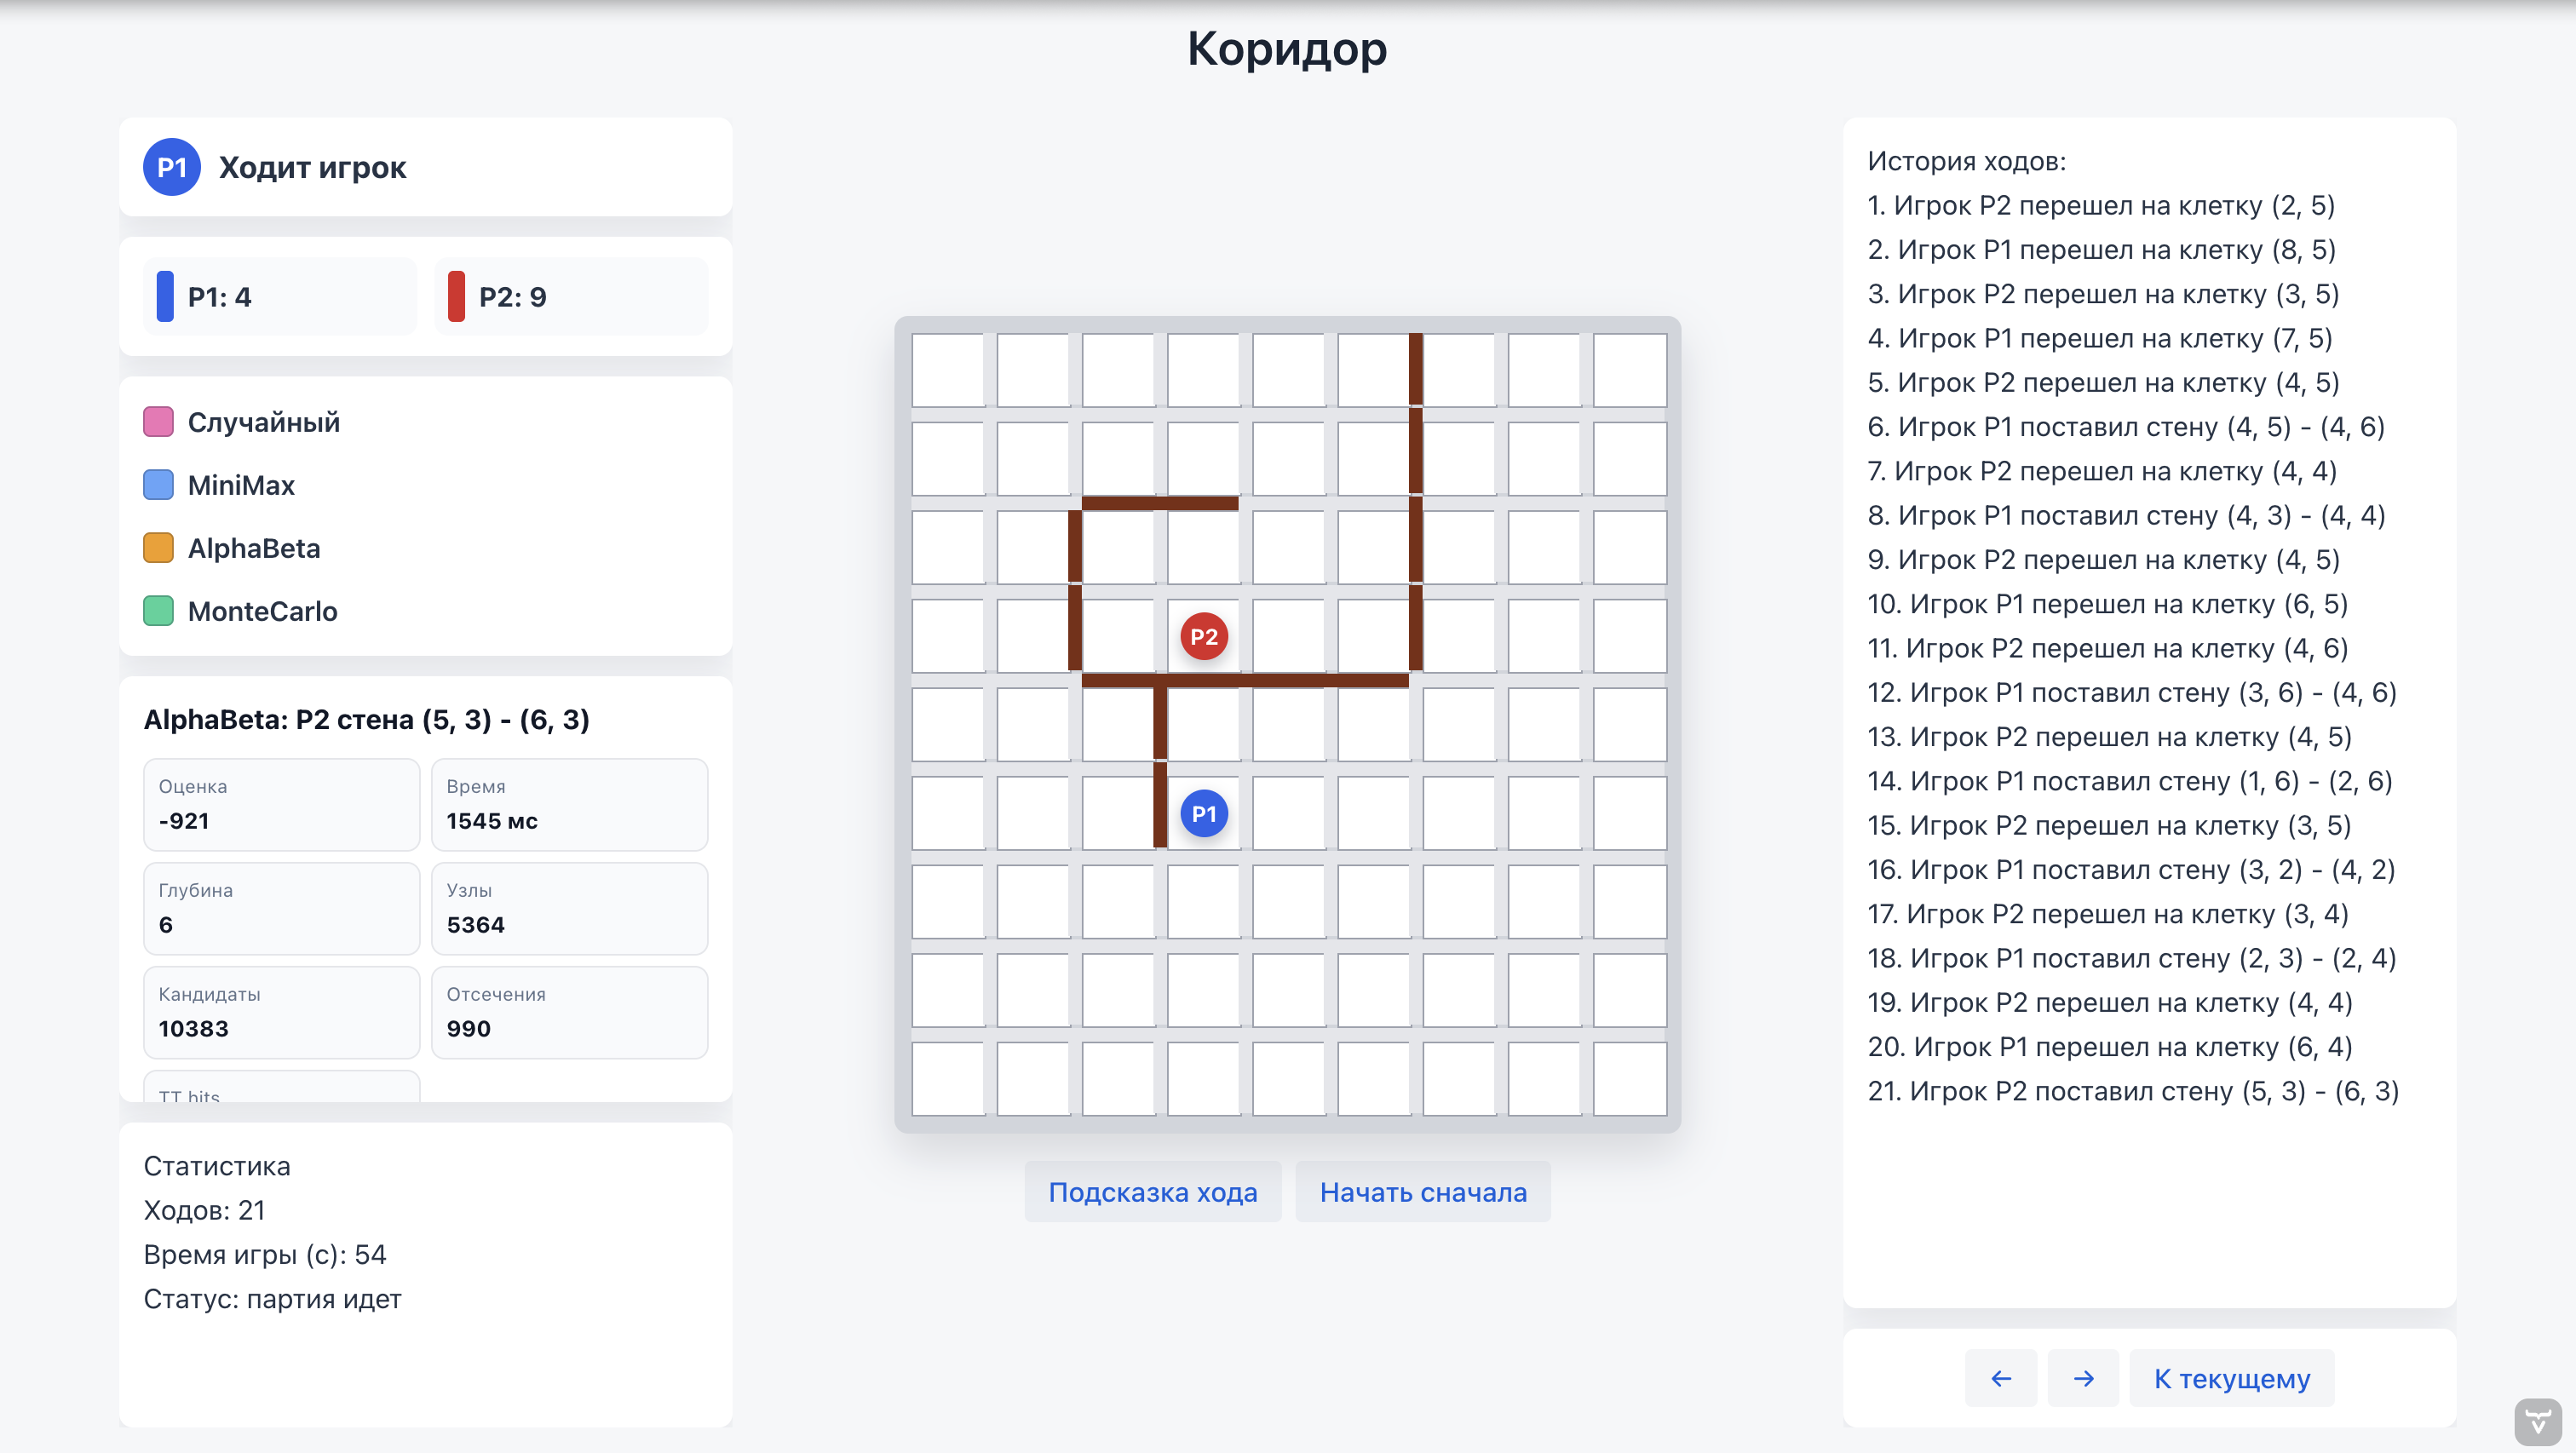
\includegraphics[width=.88\textwidth]{game-page.png}
\end{figure}
\end{frame}

\begin{frame}{Подсказки и объяснение хода}
\begin{figure}
    \centering
    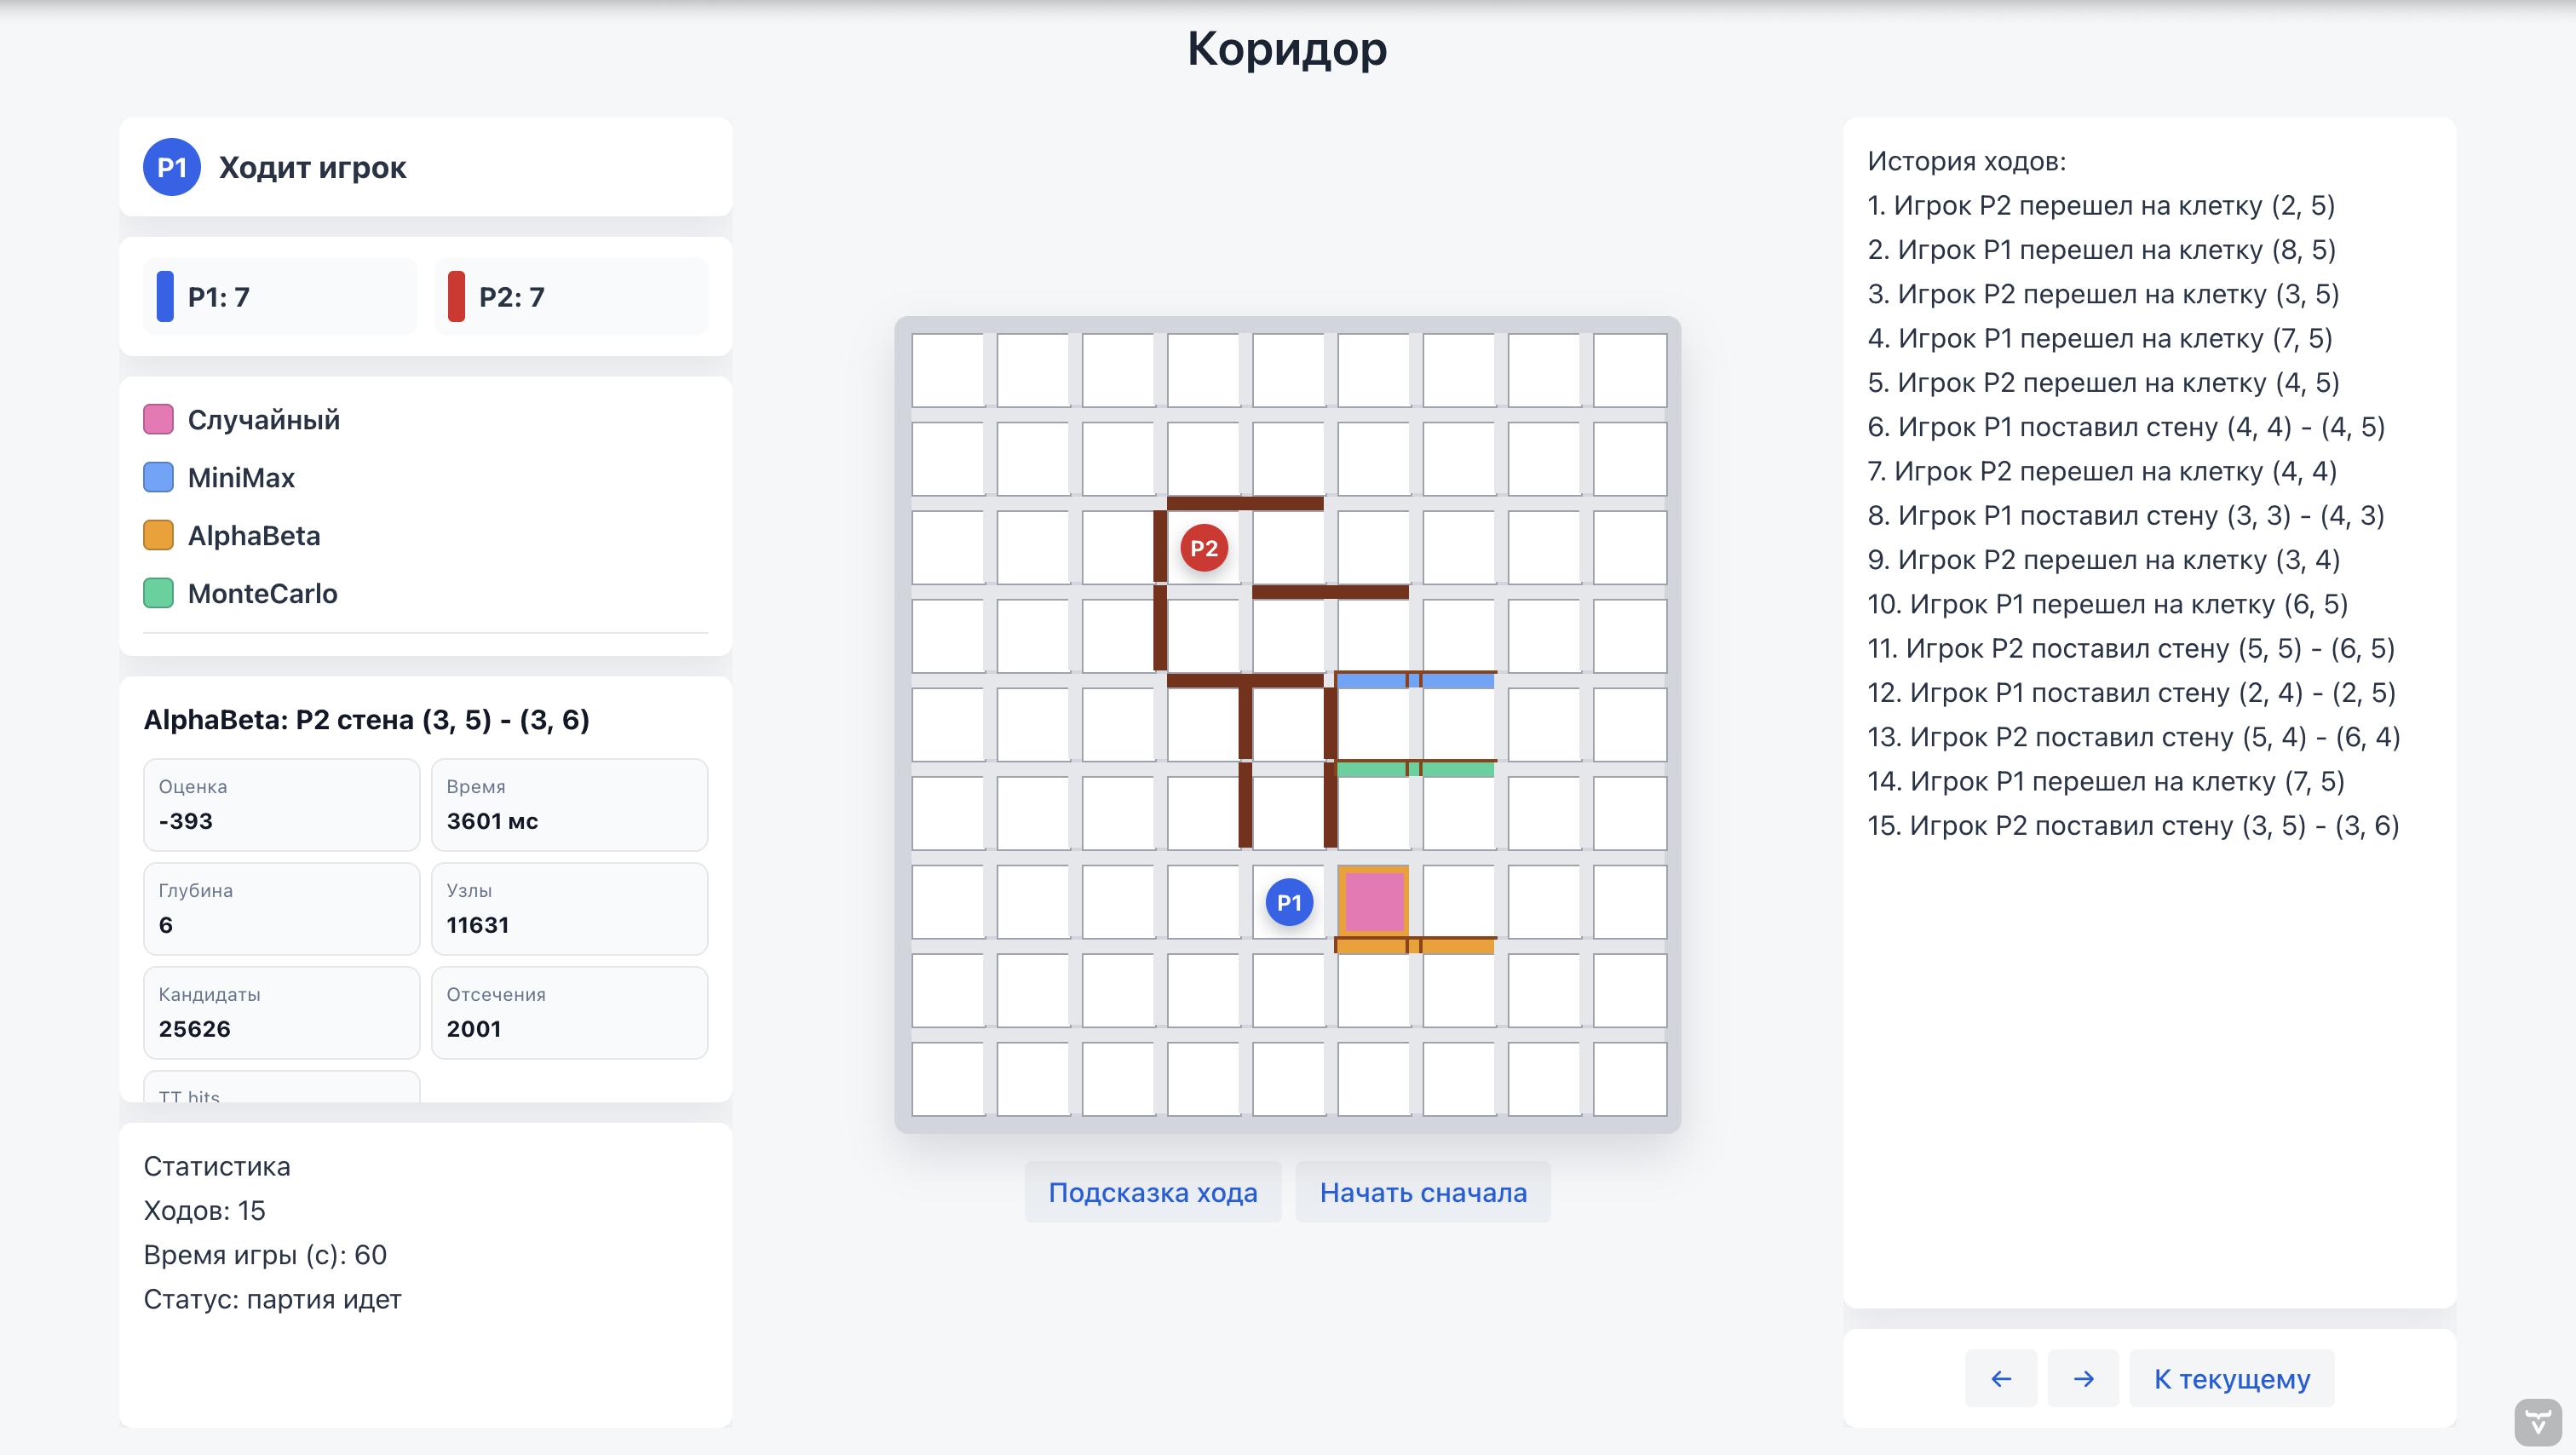
\includegraphics[width=.92\textwidth,height=.72\textheight,keepaspectratio]{hint.png}
\end{figure}
\end{frame}

\begin{frame}{Режимы автоматического сравнения}
\begin{columns}
\begin{column}{.50\textwidth}
\begin{figure}
    \centering
    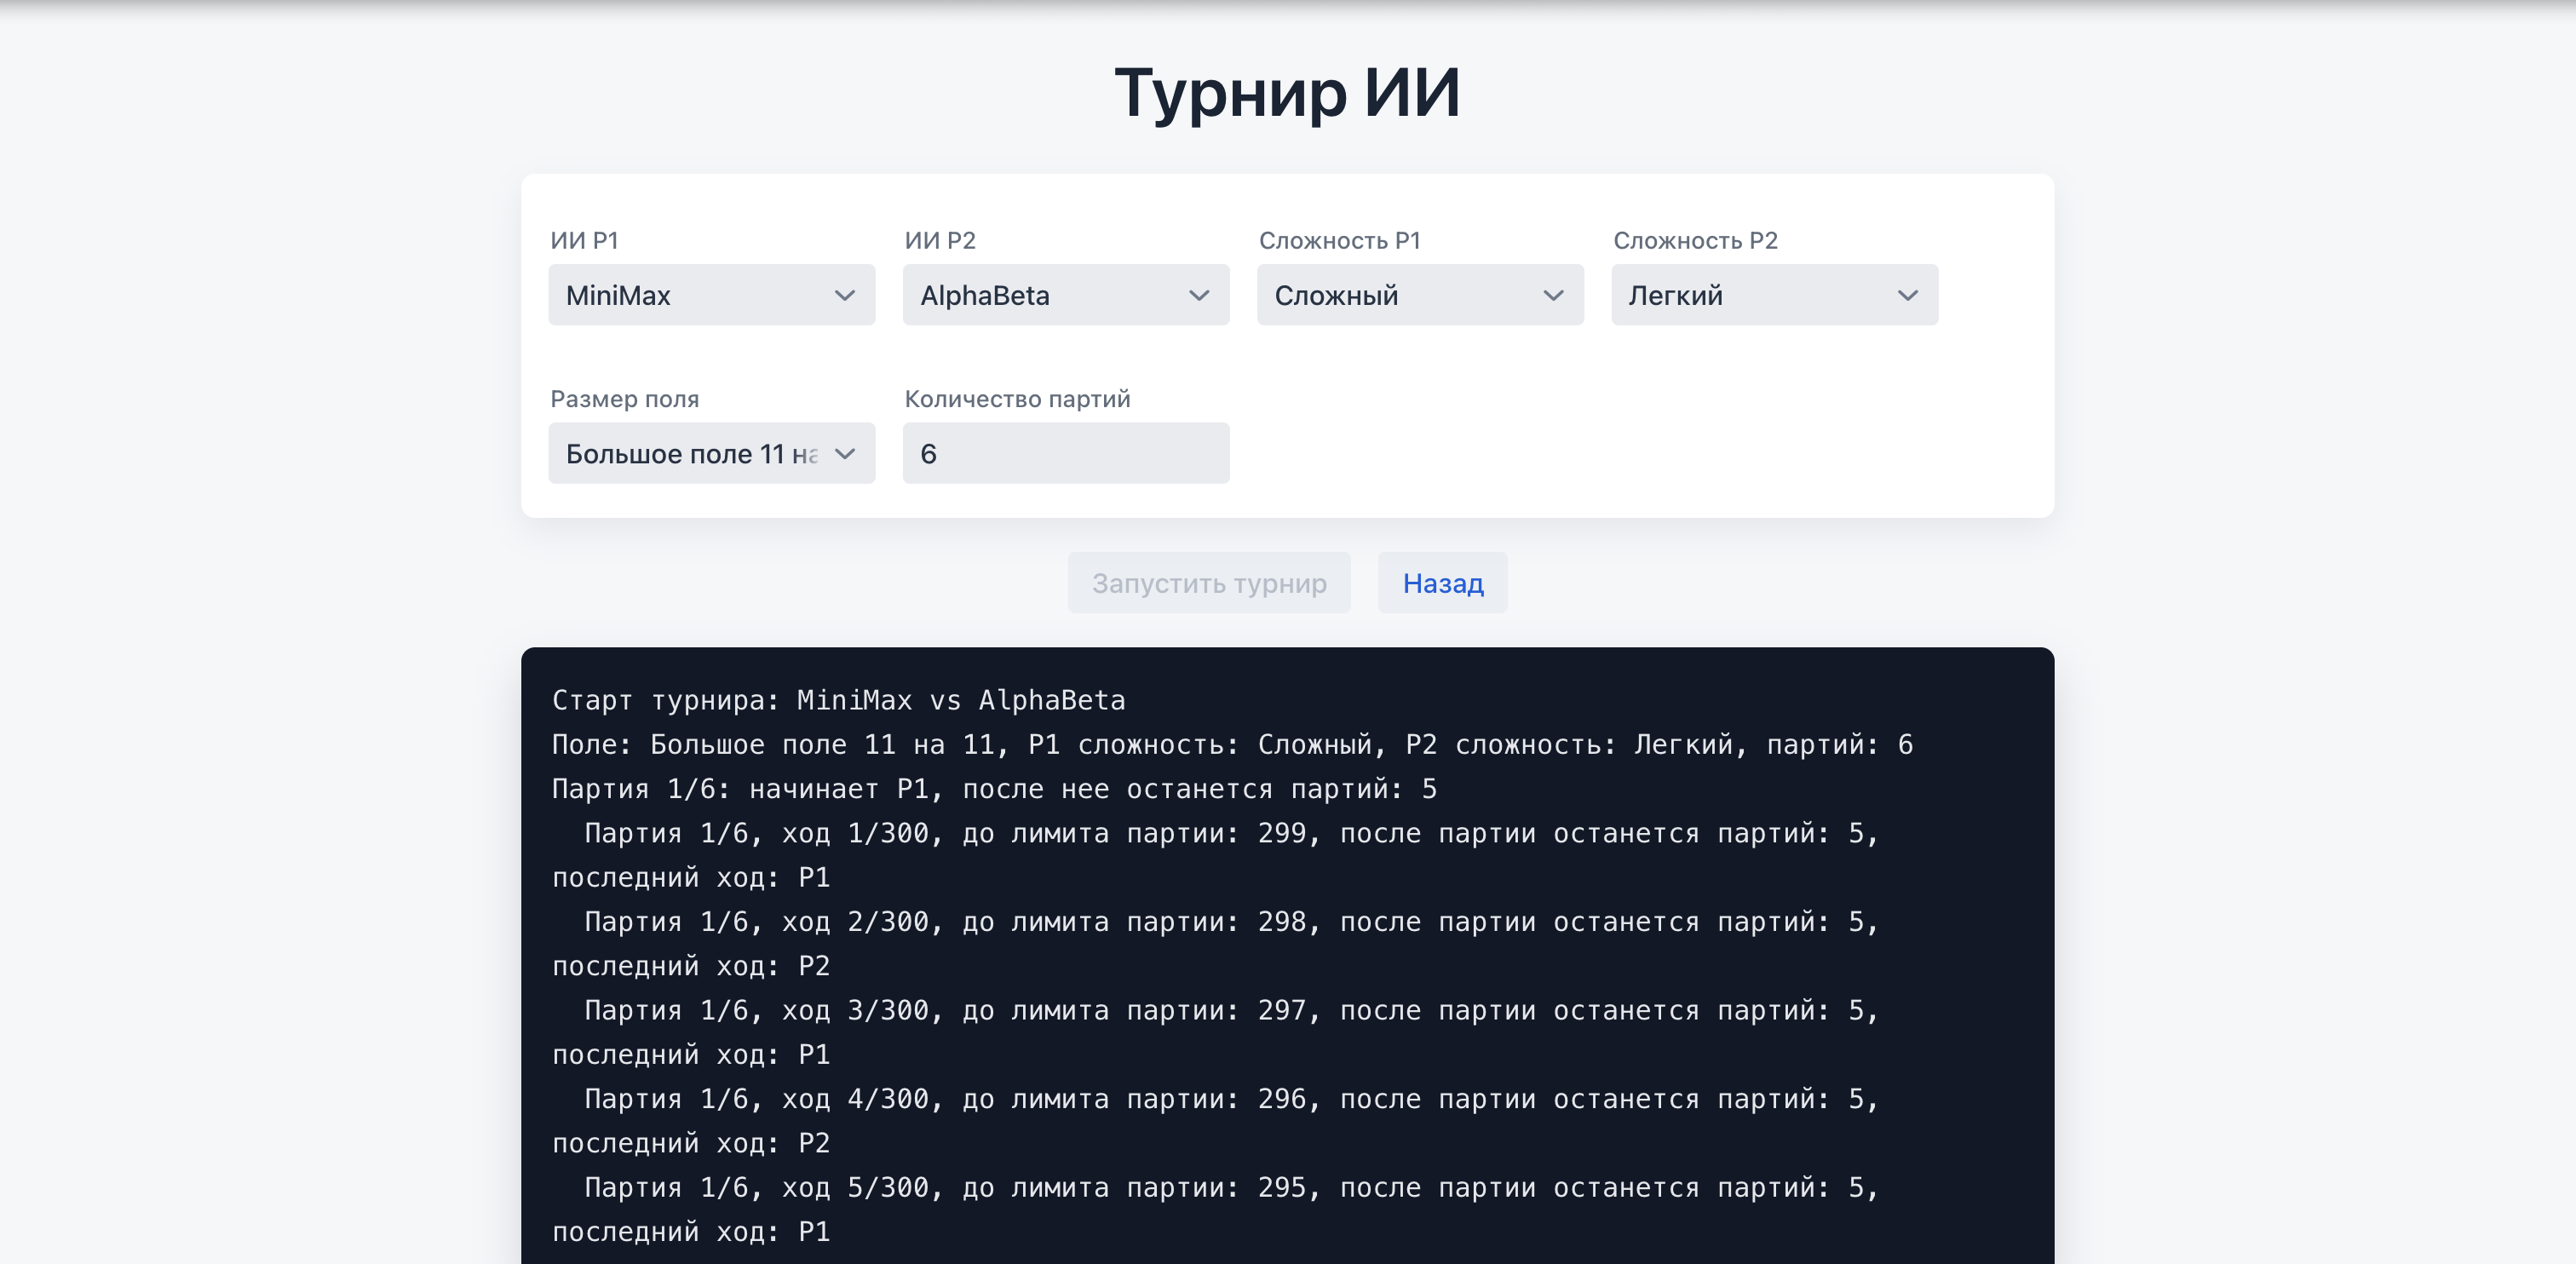
\includegraphics[width=.95\textwidth]{tournament-page.png}
\end{figure}
\end{column}
\begin{column}{.50\textwidth}
\begin{figure}
    \centering
    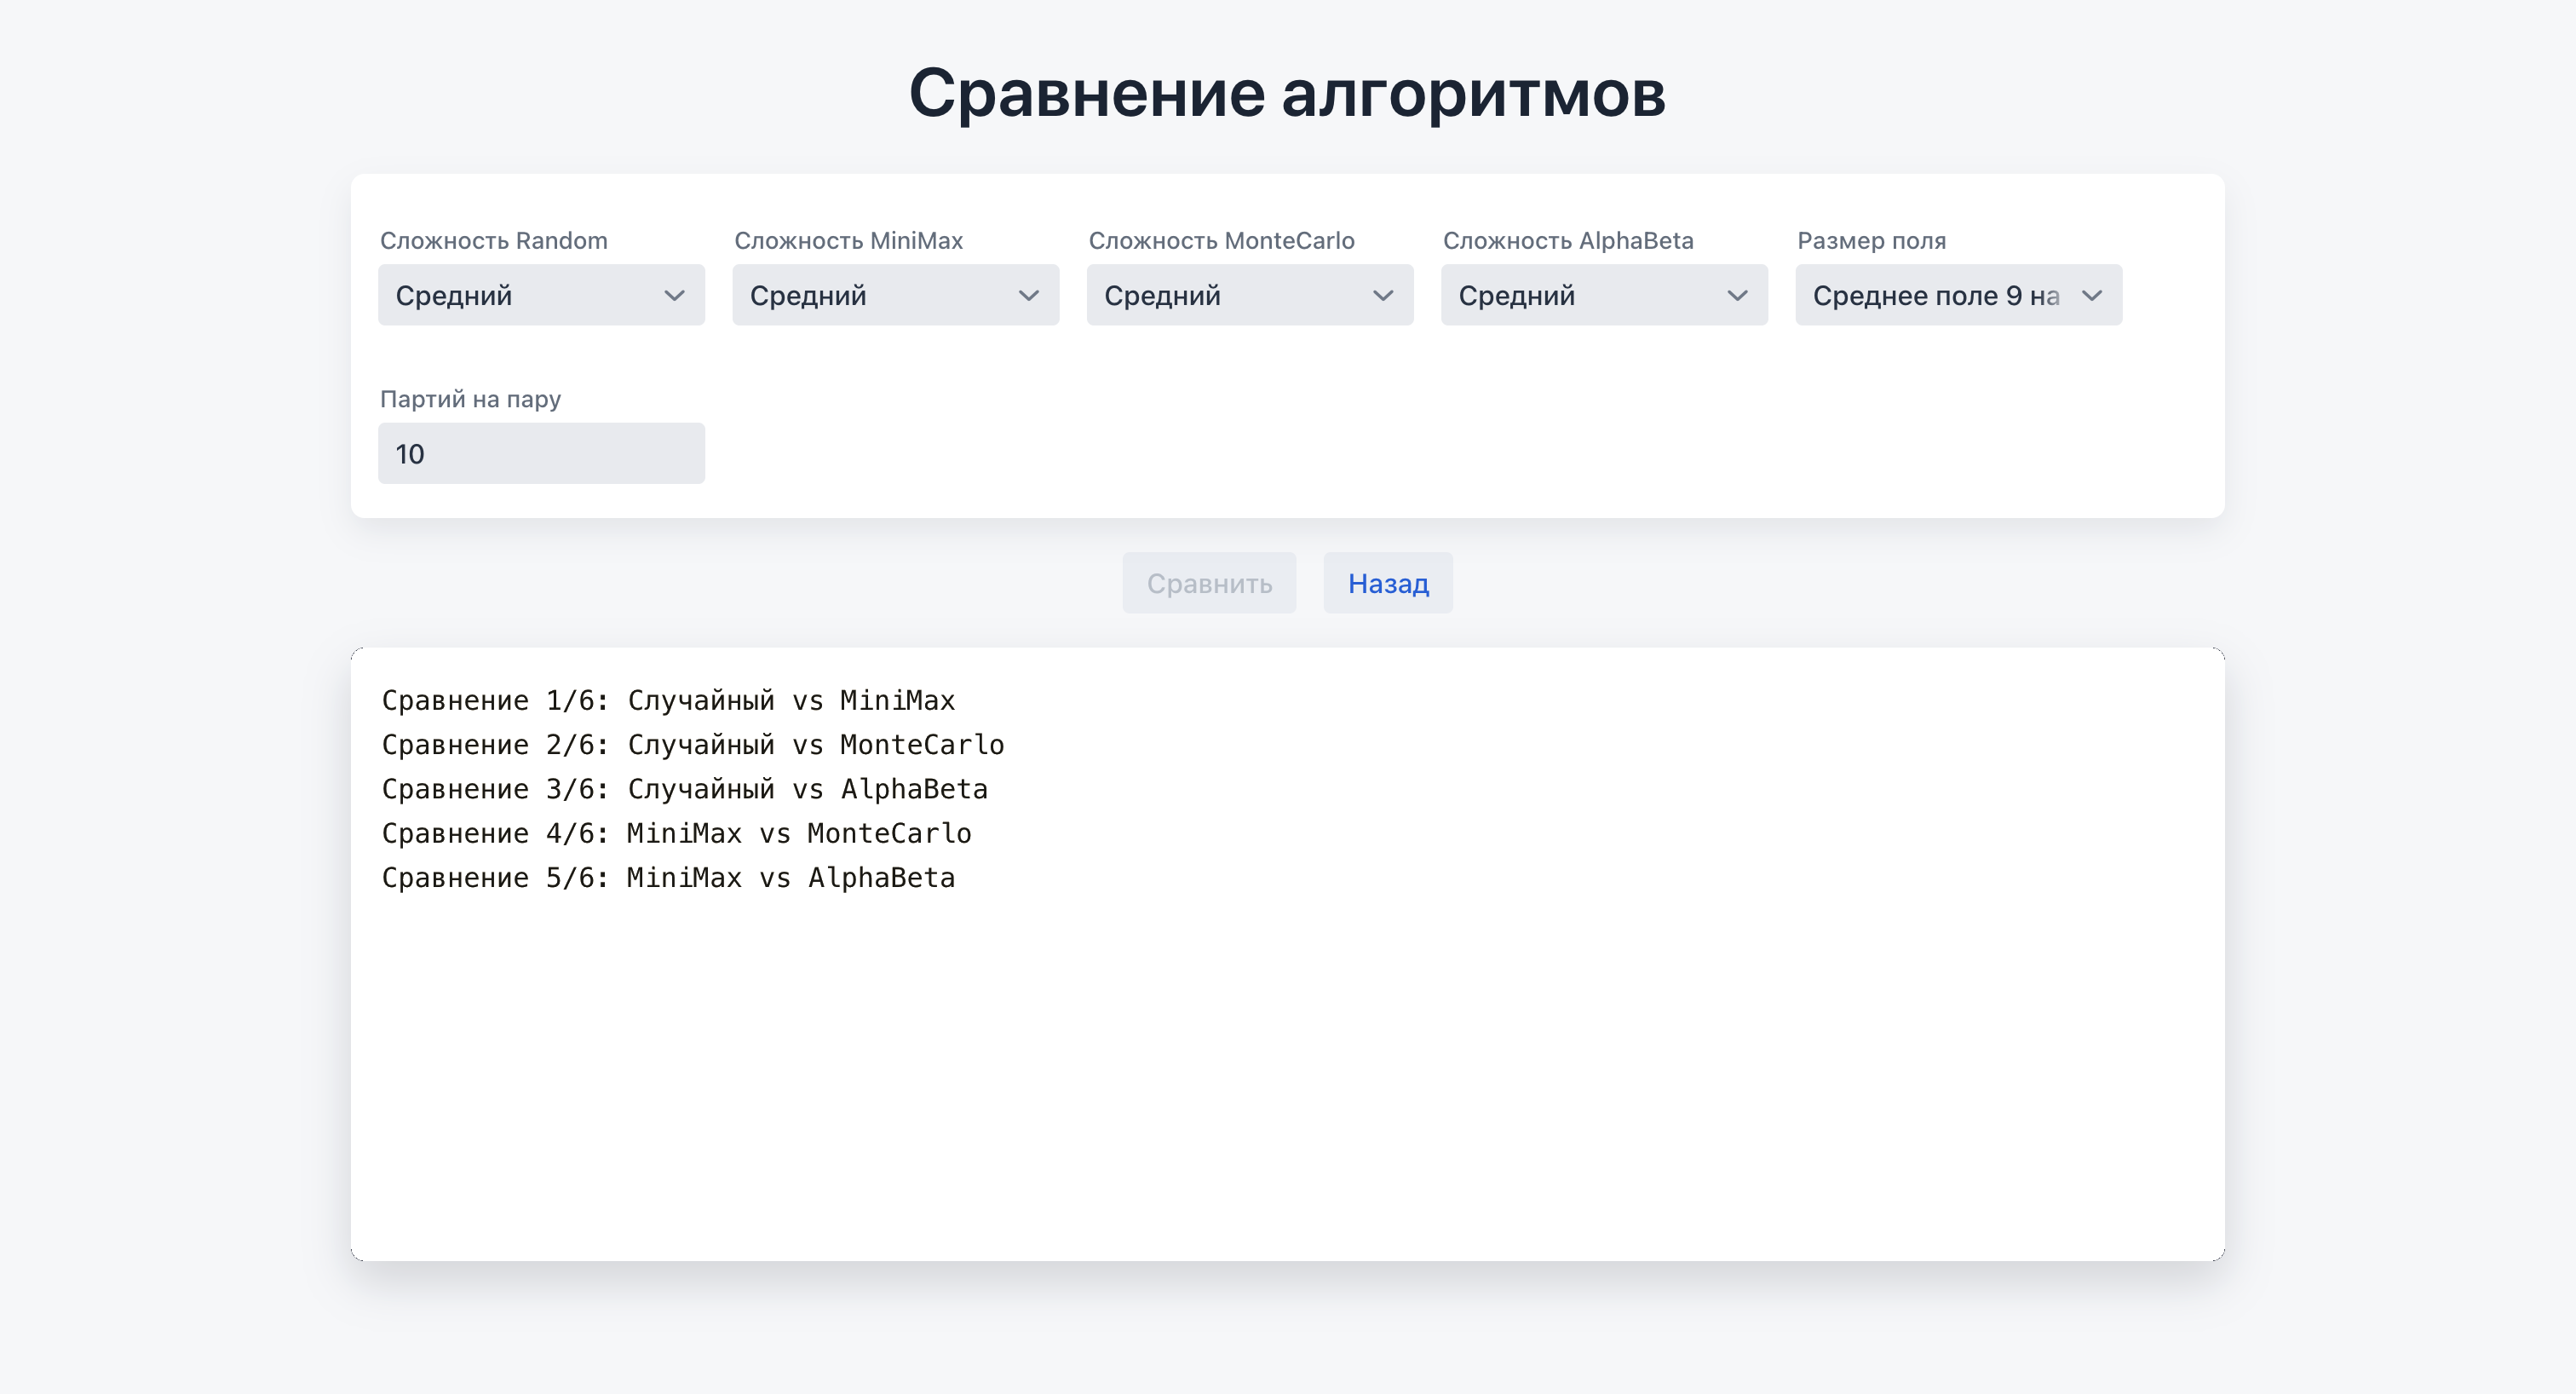
\includegraphics[width=.95\textwidth]{comparison-page.png}
\end{figure}
\end{column}
\end{columns}
\begin{block}{}
В приложении реализованы режимы турнира и сравнения алгоритмов с логами прогресса и итоговой статистикой.
\end{block}
\end{frame}

\section{Эксперимент}

\begin{frame}{Постановка эксперимента}
\begin{block}{}
    Для каждой пары алгоритмов проводились 50 партий на полях размеров $7\times7$, $9\times9$, $11\times11$. Была выбрана максимальная сложность каждого из них.
\begin{itemize}
    \item сравнивались четыре алгоритма;
    \item использовались поля $7\times7$, $9\times9$, $11\times11$;
    \item для каждой пары алгоритмов проводились автоматические партии;
    \item фиксировались победы, длина партии, время хода, глубина и число просмотренных состояний.
\end{itemize}
\end{block}

\end{frame}

\begin{frame}{Результаты: поле $7\times7$}
\begin{table}
\centering
\small
\resizebox{\textwidth}{!}{%
\begin{tabular}{lrrrrr}
\toprule
Алгоритм & Партий & Победы & Поражения & Лимит & Доля побед \\
\midrule
MiniMax    & 150 & 126 & 24  & 0 & 84,00\% \\
AlphaBeta  & 150 & 93  & 57  & 0 & 62,00\% \\
MonteCarlo & 150 & 81  & 69  & 0 & 54,00\% \\
Случайный  & 150 & 0   & 150 & 0 & 0,00\% \\
\bottomrule
\end{tabular}
}
\end{table}
\end{frame}

\begin{frame}{Результаты: поле $9\times9$}
\begin{table}
\centering
\small
\resizebox{\textwidth}{!}{%
\begin{tabular}{lrrrrr}
\toprule
Алгоритм & Партий & Победы & Поражения & Лимит & Доля побед \\
\midrule
MonteCarlo & 150 & 107 & 43  & 0 & 71,33\% \\
MiniMax    & 150 & 97  & 52  & 1 & 64,67\% \\
AlphaBeta  & 150 & 94  & 55  & 1 & 62,67\% \\
Случайный  & 150 & 0   & 148 & 2 & 0,00\% \\
\bottomrule
\end{tabular}
}
\end{table}
\end{frame}

\begin{frame}{Результаты: поле $11\times11$}
\begin{table}
\centering
\small
\resizebox{\textwidth}{!}{%
\begin{tabular}{lrrrrr}
\toprule
Алгоритм & Партий & Победы & Поражения & Лимит & Доля побед \\
\midrule
AlphaBeta  & 150 & 121 & 27  & 2 & 80,67\% \\
MonteCarlo & 150 & 88  & 59  & 3 & 58,67\% \\
MiniMax    & 150 & 84  & 62  & 4 & 56,00\% \\
Случайный  & 150 & 0   & 145 & 5 & 0,00\% \\
\bottomrule
\end{tabular}
}
\end{table}
\end{frame}

\begin{frame}{Среднее время выбора хода}
\begin{figure}
\centering
\begin{tikzpicture}[x=1.35cm,y=0.00060cm]
    \draw[->] (0,0) -- (4.8,0) node[right] {Размер};
    \draw[->] (0,0) -- (0,7200) node[above] {мс};
    \foreach \x/\label in {0/7,2/9,4/11} {
        \draw (\x,0) -- (\x,-120) node[below] {$\label\times\label$};
    }
    \foreach \y/\label in {0/0,2000/2000,4000/4000,6000/6000} {
        \draw (0,\y) -- (-0.08,\y) node[left] {\label};
        \draw[black!10] (0,\y) -- (4.2,\y);
    }
    \draw[black, thick] plot coordinates {(0,737.6) (2,935.2) (4,1578.5)};
    \draw[green!55!black, thick] plot coordinates {(0,4807.6) (2,4991.9) (4,6576.2)};
    \draw[red, thick] plot coordinates {(0,2274.3) (2,2277.5) (4,2743.9)};
    \draw[blue, thick] plot coordinates {(0,0.4) (2,0.7) (4,1.0)};
    \foreach \x/\y in {0/737.6,2/935.2,4/1578.5} \fill[black] (\x,\y) circle (2pt);
    \foreach \x/\y in {0/4807.6,2/4991.9,4/6576.2} \fill[green!55!black] (\x,\y) circle (2pt);
    \foreach \x/\y in {0/2274.3,2/2277.5,4/2743.9} \fill[red] (\x,\y) circle (2pt);
    \foreach \x/\y in {0/0.4,2/0.7,4/1.0} \fill[blue] (\x,\y) circle (2pt);
    \node[anchor=west, font=\small] at (4.35,5400) {MiniMax};
    \node[anchor=west, font=\small] at (4.35,4550) {\textcolor{green!55!black}{MonteCarlo}};
    \node[anchor=west, font=\small] at (4.35,3700) {\textcolor{red}{AlphaBeta}};
    \node[anchor=west, font=\small] at (4.35,2850) {\textcolor{blue}{Случайный}};
    \node[anchor=west, font=\scriptsize] at (4.35,2450)
        {\textcolor{blue}{}};
\end{tikzpicture}
\end{figure}
\end{frame}

\begin{frame}{Средняя длина партии}
\begin{figure}
\centering
\begin{tikzpicture}[x=1.35cm,y=0.031cm]
    \draw[->] (0,0) -- (4.8,0) node[right] {Размер};
    \draw[->] (0,0) -- (0,130) node[above] {ходов};
    \foreach \x/\label in {0/7,2/9,4/11} {
        \draw (\x,0) -- (\x,-2) node[below] {$\label\times\label$};
    }
    \foreach \y/\label in {0/0,30/30,60/60,90/90,120/120} {
        \draw (0,\y) -- (-0.08,\y) node[left] {\label};
        \draw[black!10] (0,\y) -- (4.2,\y);
    }
    \draw[blue, thick] plot coordinates {(0,58.03) (2,97.27) (4,114.87)};
    \draw[black, thick] plot coordinates {(0,46.10) (2,73.23) (4,111.43)};
    \draw[green!55!black, thick] plot coordinates {(0,58.70) (2,97.37) (4,120.27)};
    \draw[red, thick] plot coordinates {(0,45.70) (2,96.67) (4,97.17)};
    \foreach \x/\y in {0/58.03,2/97.27,4/114.87} \fill[blue] (\x,\y) circle (2pt);
    \foreach \x/\y in {0/46.10,2/73.23,4/111.43} \fill[black] (\x,\y) circle (2pt);
    \foreach \x/\y in {0/58.70,2/97.37,4/120.27} \fill[green!55!black] (\x,\y) circle (2pt);
    \foreach \x/\y in {0/45.70,2/96.67,4/97.17} \fill[red] (\x,\y) circle (2pt);
    \node[anchor=west, font=\small] at (4.35,116) {\textcolor{blue}{Случайный}};
    \node[anchor=west, font=\small] at (4.35,104) {MiniMax};
    \node[anchor=west, font=\small] at (4.35,92) {\textcolor{green!55!black}{MonteCarlo}};
    \node[anchor=west, font=\small] at (4.35,80) {\textcolor{red}{AlphaBeta}};
\end{tikzpicture}
\end{figure}
\end{frame}

\section{Заключение}

\begin{frame}{Заключение}
\begin{block}{Результаты работы}
\begin{itemize}
    \item разработано игровое приложение <<Коридор>>;
    \item реализованы правила игры и проверка достижимости целей;
    \item реализованы четыре алгоритма программного соперника;
    \item добавлены режимы игры против ИИ, ИИ против ИИ, турнира, сравнения и подсказки;
    \item проведено экспериментальное сравнение алгоритмов, в рамках которого наиболее эффективным себя показал AlphaBeta.
\end{itemize}
\end{block}
\end{frame}


\begin{frame}{Литература}
\begin{thebibliography}{9}
\bibitem{Russell:2021}
Russell, S., Norvig, P.
\newblock Artificial Intelligence: A Modern Approach. "--- Pearson, 2021.
\bibitem{Berlekamp:2001}
Berlekamp, E.R., Conway, J.H., Guy, R.K.
\newblock Winning Ways for Your Mathematical Plays. "--- A K Peters, 2001.
\bibitem{Respall:2018}
Massague Respall, V., Brown, J.A., Aslam, H.
\newblock Monte Carlo Tree Search for Quoridor. "--- 2018.
\bibitem{Jose:2022}
Moskowitz, B., Joseph, J.
\newblock Quoridor-AI. "--- 2022.
\end{thebibliography}
\end{frame}

\begin{frame}{}
\begin{center}
\vspace{1.2cm}
{\LARGE Спасибо за внимание!}

\vspace{.8cm}
\end{center}
\end{frame}

\begin{frame}{Скачать приложение}
\begin{center}
\vspace{.8cm}
{\Large Архивы приложения для Windows и macOS}

\vspace{.6cm}
{\large \url{https://github.com/karpuninaleksandr/quoridor/releases}}

\vspace{.6cm}
\small
В релизах доступны архивы с готовой сборкой приложения.
\end{center}
\end{frame}

\end{document}
